\section{Технический проект}
\subsection{Общая характеристика организации решения задачи}

Необходимо спроектировать и разработать веб-платформу, направленную на продвижение и оптимизацию деятельности компании на рынке.

Интернет-платформа представляет собой совокупность взаимосвязанных веб-сервисов, доступных через единый пользовательский интерфейс. Каждый сервис представляет собой отдельный функциональный модуль, содержащий текстовую, графическую, а также мультимедийную информацию (видеоконференции, изображения, файлы и т.д.).

Веб-платформа и её веб-сервисы будут размещены в сети Интернет по определённому доменному имени (например, https://calendar.mycompany.ru, https://talks.mycompany.ru, https://mail.mycompany.ru и т.д.). Каждая страница платформы реализуется с использованием современных веб-технологий: HTML, CSS, JavaScript (React) и других, а также может использовать фреймворки и библиотеки для обеспечения адаптивности, интерактивности и высокой производительности.

\subsection{Обоснование выбора технологии проектирования}

На сегодняшний день информационный рынок, поставляющий программные решения в выбранной сфере, предлагает множество продуктов, позволяющих достигнуть поставленной цели – разработки веб-платформы.

\subsubsection{Описание используемых языков программирования}

В процессе разработки веб-платформы используются программные средства и языки программирования. Каждое программное средство и каждый язык программирования применяется для круга задач, при решении которых они необходимы.

\subsubsection{Язык программирования Python}

Python — это высокоуровневый язык программирования общего назначения с поддержкой нескольких парадигм, включая объектно-ориентированное, процедурное и функциональное программирование. Благодаря своей простоте, читаемости и обширной экосистеме библиотек, Python широко применяется в разработке веб-приложений, автоматизации процессов, анализе данных, машинном обучении и многих других областях. В контексте разработки веб-приложений Python используется совместно с фреймворками, такими как Django и Flask, которые обеспечивают удобные средства для создания серверной логики, обработки запросов и генерации динамических веб-страниц.

\subsubsection{Язык программирования JavaScript}

\paragraph{Достоинства языка JavaScript}

JavaScript — это высокоуровневый интерпретируемый язык программирования, основной задачей которого является создание интерактивного поведения на веб-страницах. Он является неотъемлемой частью технологии разработки клиентской части веб-приложений и поддерживается всеми современными веб-браузерами. С помощью JavaScript можно реализовывать динамическое обновление содержимого, проверку данных на стороне клиента, обработку событий, а также взаимодействие с сервером без перезагрузки страницы (через AJAX-запросы). Современные стандарты JavaScript (начиная с ECMAScript 6) предоставляют широкий набор возможностей, включая модули, асинхронные функции, классы и работу с промисами. Для повышения совместимости и ускорения разработки часто используются библиотеки и фреймворки, такие как jQuery, React, Vue.js и другие. Они позволяют упростить доступ к элементам DOM, реализовать реактивные интерфейсы и обеспечить кроссбраузерную поддержку. JavaScript выполняется непосредственно в браузере пользователя, что позволяет создавать отзывчивые и интерактивные пользовательские интерфейсы без необходимости постоянной связи с сервером.

\paragraph{Недостатки языка JavaScript}

\begin{itemize}
  \item parseInt("08") // → 0
  \item parseInt("0x10") // → 16
  \item parseInt("0x10", 10) // → 0
  \item null == 0 // → false
  \item null > 0 // → false
  \item null >= 0 // → true
  \item undefined == null // → true
  \item undefined === null // → false
  \item typeof NaN // → "number"
  \item NaN === NaN // → false
  \item "5" + 3 // → "53"
  \item "5" - 3 // → 2
  \item "5" * "3" // → 15
  \item "5" * "abc" // → NaN
  \item 0.1 + 0.2 === 0.3 // → false
  \item (0.1 + 0.2).toFixed(1) // → "0.3"
  \item true + true // → 2
  \item true - false // → 1
  \item "1" + true // → "1true"
  \item "1" - true // → 0
\end{itemize}

\subsubsection{React}
React — это популярная JavaScript-библиотека для создания пользовательских интерфейсов. Она позволяет строить интерактивные веб-приложения с помощью компонентного подхода.

Основные преимущества React:
\begin{itemize}
\item Виртуальный DOM для эффективного обновления интерфейса
\item Компонентная архитектура, способствующая повторному использованию кода
\item Односторонний поток данных, упрощающий отладку приложений
\item Богатая экосистема дополнительных библиотек и инструментов
\item Поддержка серверного рендеринга (Next.js)
\end{itemize}

В нашем проекте React используется для построения клиентской части всех веб-сервисов платформы. Это позволяет создавать единообразные, отзывчивые интерфейсы с высокой производительностью.

\subsubsection{Apache James и JMAP}
Apache James — это open-source почтовый сервер, написанный на Java. Он предоставляет полный набор почтовых протоколов (SMTP, POP3, IMAP) и может использоваться как самостоятельное решение или как часть более крупной системы.

JMAP (JSON Meta Application Protocol) — современный протокол для работы с почтой, календарями и контактами, призванный заменить устаревшие IMAP и SMTP. Его преимущества:
\begin{itemize}
\item Использование JSON для передачи данных
\item Эффективная синхронизация состояния
\item Поддержка push-уведомлений
\item Единый API для почты, календарей и контактов
\end{itemize}

В нашей платформе мы используем Apache James с поддержкой JMAP для реализации почтового сервиса, что обеспечивает:
\begin{itemize}
\item Надежную доставку и хранение почты
\item Быструю синхронизацию между клиентами
\item Современный API для интеграции с другими сервисами
\end{itemize}

\subsubsection{Node.js}
Node.js — это серверная платформа для выполнения JavaScript, построенная на движке V8. Она использует событийно-ориентированную, неблокирующую модель ввода-вывода, что делает её легковесной и эффективной.

Основные особенности Node.js, используемые в нашем проекте:
\begin{itemize}
\item Высокая производительность для I/O-интенсивных операций
\item Единая языковая среда для клиента и сервера (JavaScript)
\item Богатая экосистема пакетов (npm)
\item Поддержка современных стандартов JavaScript
\end{itemize}

В нашей архитектуре Node.js используется для:
\begin{itemize}
\item Реализации серверной логики некоторых микросервисов
\item Обработки реального времени (чаты, уведомления)
\item Серверного рендеринга React-приложений
\item Построения API-шлюза для объединения различных сервисов
\end{itemize}

Сочетание этих технологий позволяет нам создать масштабируемую, производительную платформу с современным пользовательским интерфейсом и надежной серверной частью.

\subsection{Диаграмма компонентов}

Диаграмма компонентов отображает взаимодействие пользователя с сервисами. Основными элементами диаграммы являются компоненты (сервисы).

\begin{figure}[H]
\center{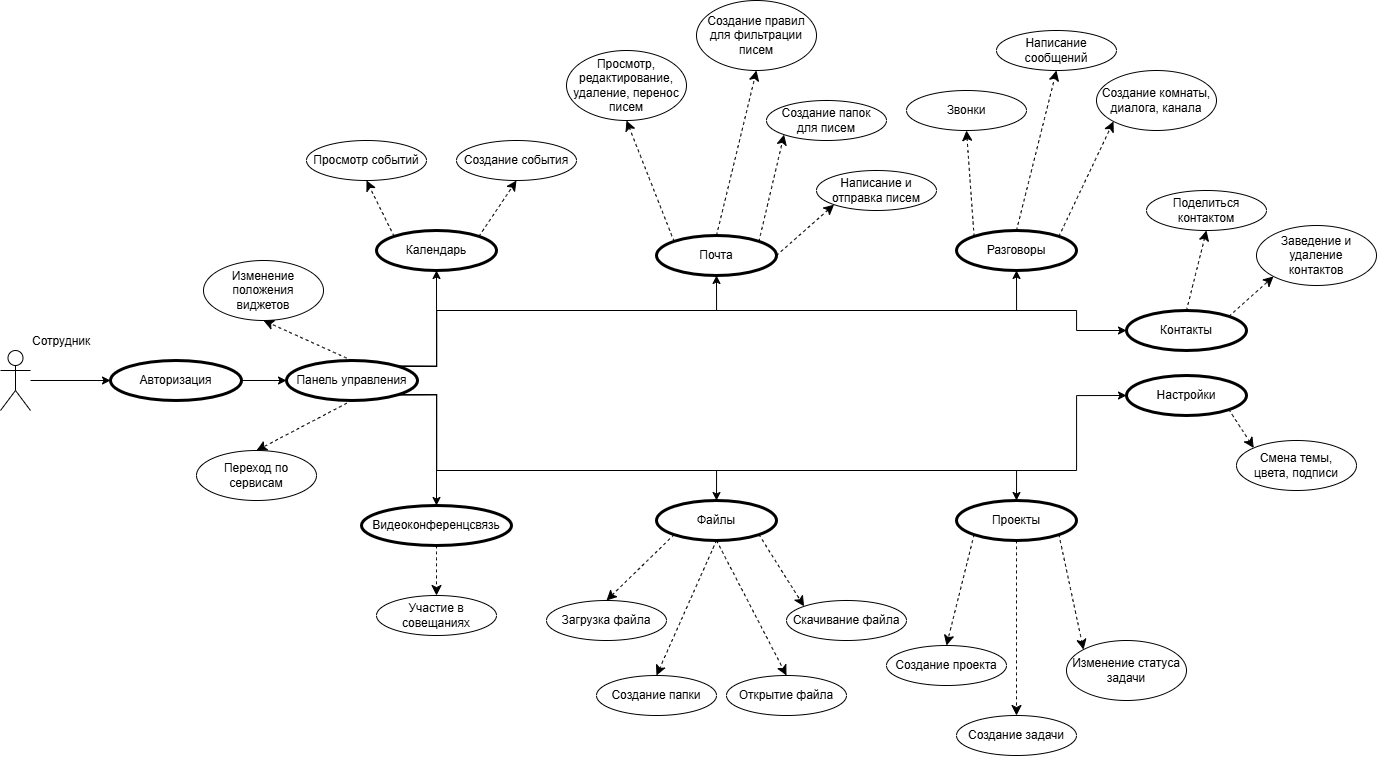
\includegraphics[width=1\linewidth]{images/diag2}}
\caption{Диаграмма компонентов}
\label{comp:image}
\end{figure}

После авторизации в веб-платформе пользователь переходит на главную рабочую страницу <<Панель управления>>, где отображаются виджеты различных сервисов.

\begin{itemize}
    \item Сервис <<Почта>> — пользователь может просматривать свои письма, отвечать на них, а также отправлять новые письма. В сервисе отображаются последние 10 входящих писем из папки Входящие. Пользователь может выбрать получателя из списка контактов и отправить письмо. Также сервис интегрирован с функцией звонков, и при наличии соответствующей кнопки в письме пользователь может совершить звонок через сервис <<Разговоры>>.
    
    \item Сервис <<Файлы>> — в этом сервисе пользователь может загружать, хранить и управлять своими файлами. Он может поделиться файлами с другими пользователями, выбрав их из списка контактов. Пользователь может настраивать права доступа для каждого файла, например, на скачивание или редактирование.

    \item Сервис <<Контакты>> — сервис предоставляет пользователю возможность управлять списком своих контактов. Он может быстро находить пользователей для отправки писем, звонков или назначения задач. В сервисе можно просматривать информацию о контактах, включая их статус и доступные способы связи.

    \item Сервис <<Разговоры>> — этот сервис позволяет пользователю совершать голосовые или видеозвонки с людьми из списка контактов. Пользователь может выбрать способ связи (текстовый чат, голосовой или видеозвонок) и начать общение. Сервис интегрируется с почтовым сервисом, позволяя удобно начинать звонки после переписки по почте.

    \item Сервис <<Задачи>> — в этом сервисе пользователь может назначать задачи другим пользователям, выбрав их из списка контактов. Задачи могут быть связаны с проектами или обычными делами. Пользователь может отслеживать состояние задач (выполнена, в процессе и т.д.) и получать уведомления о статусе задач.

    \item Сервис <<Видеоконференцсвязь>> — в этом сервисе пользователь может создавать или присоединяться к видеоконференциям. Он может приглашать участников, проводить видеозвонки и использовать функции обмена экранами и чатом во время конференции.

    \item Сервис <<Календарь>> — сервис календаря позволяет пользователю планировать свои события и задачи. Пользователь может добавлять мероприятия, настраивать напоминания и получать уведомления о предстоящих событиях. Календарь интегрируется с задачами, и пользователь может добавлять задачи в календарь для более удобного планирования.

    \item Сервис <<Настройки>> — в этом сервисе пользователь может настроить параметры своей учетной записи, такие как изменение личной информации, настройка уведомлений, конфиденциальности и безопасности. Также можно выбрать тему оформления интерфейса (светлая или темная) и язык платформы.
\end{itemize}

\subsection{Диаграмма размещения}

Диаграмма размещения (рис.~\ref{place:image}) отражает физические взаимосвязи между программными и аппаратными компонентами системы.

\vspace{-8mm} % чтобы убрать пустую строку, которая осталась после переноса рисунка на следующую страницу
\begin{figure}[H]
\center{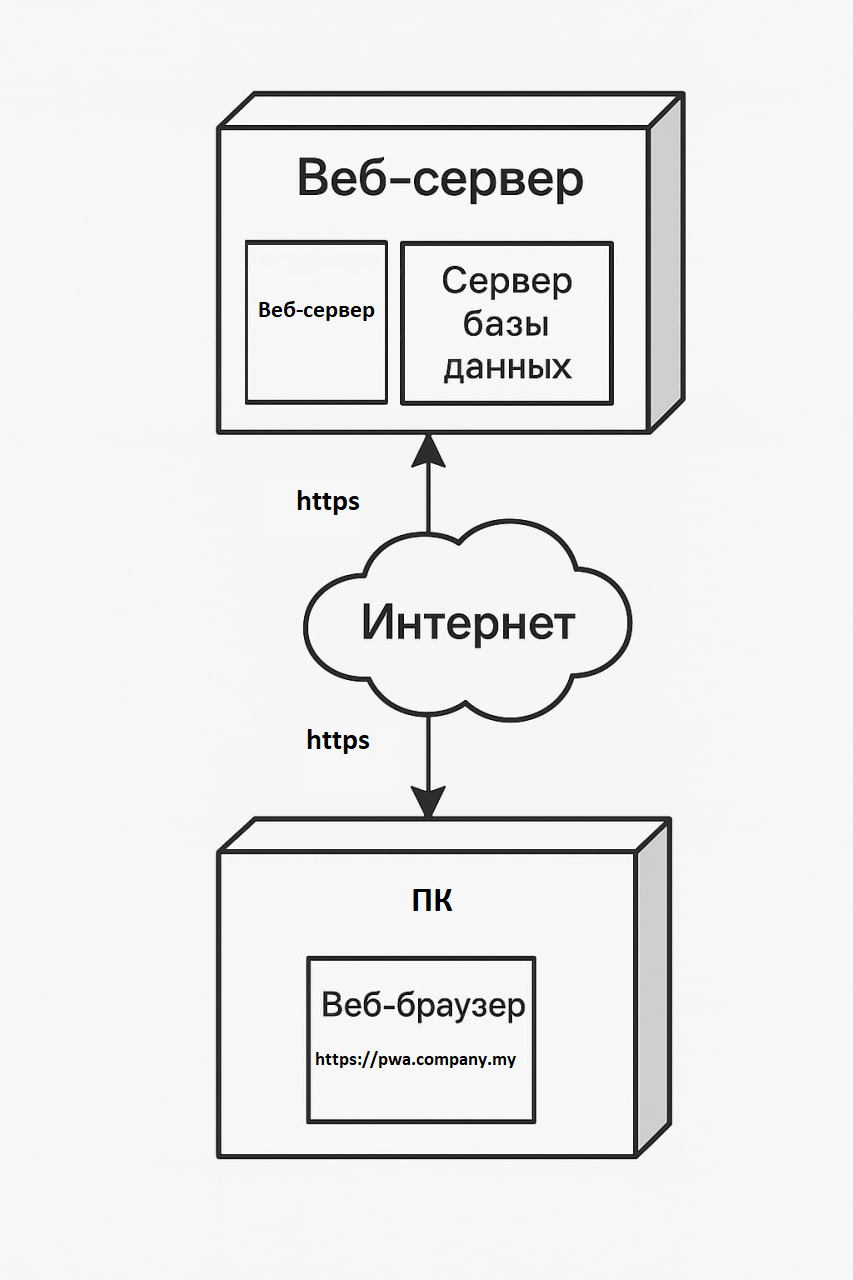
\includegraphics[width=0.57\linewidth]{images/диаграмма2}}
\caption{Диаграмма размещения}
\label{place:image}
\end{figure}

\subsection{Содержание информационных блоков. Основные сущности}

Проанализировав требования, можно выделить следующие основные сущности:
\begin{itemize}
  \item "<Почта">;
  \item "<Видеоконференцсвязь">;
  \item "<Календарь">;
  \item "<Панель управления">;
  \item "<Контакты">;
  \item "<Настройки">;
  \item "<Проекты">;
  \item "<Разговоры">;
  \item "<Файлы">.
\end{itemize}

В состав сущностей входят следующие атрибуты:

\begin{xltabular}{\textwidth}{|l|l|p{3.2cm}|X|}
  \caption{Атрибуты сущности "<Почта">\label{mail:table}}\\ \hline
  Поле & Тип & Обязательное & Описание \\ \hline
  \endfirsthead
  \continuecaption{Продолжение таблицы \ref{mail:table}}\\ \hline
  Поле & Тип & Обязательное & Описание \\ \hline
  \endhead
  id & ObjectId & true & Уникальный идентификатор письма \\ \hline
  sender & String & true & Отправитель \\ \hline
  recipients & Array[String] & true & Получатели \\ \hline
  subject & String & false & Тема письма \\ \hline
  body & String & false & Текст письма \\ \hline
  attachments & Array & false & Список вложений \\ \hline
  timestamp & Date & true & Дата и время отправки \\ \hline
  read & Boolean & true & Признак прочтения \\ \hline
\end{xltabular}

\begin{xltabular}{\textwidth}{|l|l|p{3.2cm}|X|}
  \caption{Атрибуты сущности "<Видеоконференцсвязь">\label{video:table}}\\ \hline
  Поле & Тип & Обязательное & Описание \\ \hline
  \endfirsthead
  \continuecaption{Продолжение таблицы \ref{video:table}}\\ \hline
  Поле & Тип & Обязательное & Описание \\ \hline
  \endhead
  id & ObjectId & true & Уникальный идентификатор конференции \\ \hline
  participants & Array[String] & true & Участники \\ \hline
  startTime & DateTime & true & Время начала \\ \hline
  endTime & DateTime & false & Время окончания \\ \hline
  status & String & true & Статус (запланирована, активна, завершена) \\ \hline
\end{xltabular}

\begin{xltabular}{\textwidth}{|l|l|p{3.2cm}|X|}
  \caption{Атрибуты сущности "<Календарь">\label{calendar:table}}\\ \hline
  Поле & Тип & Обязательное & Описание \\ \hline
  \endfirsthead
  \continuecaption{Продолжение таблицы \ref{calendar:table}}\\ \hline
  Поле & Тип & Обязательное & Описание \\ \hline
  \endhead
  id & ObjectId & true & Уникальный идентификатор события \\ \hline
  title & String & true & Название события \\ \hline
  date & DateTime & true & Дата и время \\ \hline
  participants & Array[String] & false & Участники \\ \hline
  description & String & false & Описание \\ \hline
\end{xltabular}

\begin{xltabular}{\textwidth}{|l|l|p{3.2cm}|X|}
  \caption{Атрибуты сущности "<Панель управления">\label{dashboard:table}}\\ \hline
  Поле & Тип & Обязательное & Описание \\ \hline
  \endfirsthead
  \continuecaption{Продолжение таблицы \ref{dashboard:table}}\\ \hline
  Поле & Тип & Обязательное & Описание \\ \hline
  \endhead
  id & ObjectId & true & Идентификатор виджета \\ \hline
  name & String & true & Название виджета \\ \hline
  type & String & true & Тип виджета (статистика, список задач и т.д.) \\ \hline
  dataSource & String & true & Источник данных \\ \hline
\end{xltabular}

\begin{xltabular}{\textwidth}{|l|l|p{3.2cm}|X|}
  \caption{Атрибуты сущности "<Контакты">\label{contacts:table}}\\ \hline
  Поле & Тип & Обязательное & Описание \\ \hline
  \endfirsthead
  \continuecaption{Продолжение таблицы \ref{contacts:table}}\\ \hline
  Поле & Тип & Обязательное & Описание \\ \hline
  \endhead
  id & ObjectId & true & Уникальный идентификатор контакта \\ \hline
  name & String & true & Имя контакта \\ \hline
  email & String & true & Email \\ \hline
  phone & String & false & Телефон \\ \hline
  tags & Array[String] & false & Метки \\ \hline
\end{xltabular}

\begin{xltabular}{\textwidth}{|l|l|p{3.2cm}|X|}
  \caption{Атрибуты сущности "<Настройки">\label{settings:table}}\\ \hline
  Поле & Тип & Обязательное & Описание \\ \hline
  \endfirsthead
  \continuecaption{Продолжение таблицы \ref{settings:table}}\\ \hline
  Поле & Тип & Обязательное & Описание \\ \hline
  \endhead
  id & ObjectId & true & Идентификатор настройки \\ \hline
  userId & ObjectId & true & Пользователь \\ \hline
  theme & String & false & Выбранная тема \\ \hline
  language & String & false & Язык интерфейса \\ \hline
\end{xltabular}

\begin{xltabular}{\textwidth}{|l|l|p{3.2cm}|X|}
  \caption{Атрибуты сущности "<Проекты">\label{projects:table}}\\ \hline
  Поле & Тип & Обязательное & Описание \\ \hline
  \endfirsthead
  \continuecaption{Продолжение таблицы \ref{projects:table}}\\ \hline
  Поле & Тип & Обязательное & Описание \\ \hline
  \endhead
  id & ObjectId & true & Идентификатор проекта \\ \hline
  title & String & true & Название проекта \\ \hline
  description & String & false & Описание \\ \hline
  members & Array[String] & true & Участники проекта \\ \hline
  status & String & true & Текущий статус \\ \hline
\end{xltabular}

\begin{xltabular}{\textwidth}{|l|l|p{3.2cm}|X|}
  \caption{Атрибуты сущности "<Разговоры">\label{talks:table}}\\ \hline
  Поле & Тип & Обязательное & Описание \\ \hline
  \endfirsthead
  \continuecaption{Продолжение таблицы \ref{talks:table}}\\ \hline
  Поле & Тип & Обязательное & Описание \\ \hline
  \endhead
  id & ObjectId & true & Идентификатор беседы \\ \hline
  participants & Array[String] & true & Участники \\ \hline
  messages & Array & true & Сообщения \\ \hline
  lastMessage & String & false & Последнее сообщение \\ \hline
  unreadCount & Integer & true & Количество непрочитанных \\ \hline
\end{xltabular}

\begin{xltabular}{\textwidth}{|l|l|p{3.2cm}|X|}
  \caption{Атрибуты сущности "<Файлы">\label{files:table}}\\ \hline
  Поле & Тип & Обязательное & Описание \\ \hline
  \endfirsthead
  \continuecaption{Продолжение таблицы \ref{files:table}}\\ \hline
  Поле & Тип & Обязательное & Описание \\ \hline
  \endhead
  id & ObjectId & true & Идентификатор файла \\ \hline
  name & String & true & Название файла \\ \hline
  owner & String & true & Владелец \\ \hline
  sharedWith & Array[String] & false & Список, с кем поделились \\ \hline
  size & Integer & true & Размер в байтах \\ \hline
  createdAt & Date & true & Дата загрузки \\ \hline
\end{xltabular}

Экземпляры этих сущностей реализуются в информационных блоках пользовательского интерфейса. Атрибуты сущностей отображаются в полях, свойствах и компонентах соответствующих элементов.
